\documentclass[12pt, spanish]{article}
\usepackage[spanish]{babel}
\selectlanguage{spanish}
%\usepackage{natbib}
\usepackage{url}
\usepackage[utf8x]{inputenc}
\usepackage{graphicx}
\graphicspath{{images/}}
\usepackage{parskip}
\usepackage{fancyhdr}
\usepackage{vmargin}
\usepackage{multirow}
\usepackage{float}
\usepackage{chngpage}

\usepackage{amsfonts}

\usepackage{subcaption}

\usepackage{hyperref}
\usepackage[
    type={CC},
    modifier={by-nc-sa},
    version={4.0},
]{doclicense}

\hypersetup{
    colorlinks=true,
    linkcolor=blue,
    filecolor=magenta,      
    urlcolor=cyan,
}

% para codigo
\usepackage{listings}
\usepackage{xcolor}



%% configuración de listings

\definecolor{listing-background}{HTML}{F7F7F7}
\definecolor{listing-rule}{HTML}{B3B2B3}
\definecolor{listing-numbers}{HTML}{B3B2B3}
\definecolor{listing-text-color}{HTML}{000000}
\definecolor{listing-keyword}{HTML}{435489}
\definecolor{listing-identifier}{HTML}{435489}
\definecolor{listing-string}{HTML}{00999A}
\definecolor{listing-comment}{HTML}{8E8E8E}
\definecolor{listing-javadoc-comment}{HTML}{006CA9}

\lstdefinestyle{eisvogel_listing_style}{
  language         = python,
%$if(listings-disable-line-numbers)$
%  xleftmargin      = 0.6em,
%  framexleftmargin = 0.4em,
%$else$
  numbers          = left,
  xleftmargin      = 0em,
 framexleftmargin = 0em,
%$endif$
  backgroundcolor  = \color{listing-background},
  basicstyle       = \color{listing-text-color}\small\ttfamily{}\linespread{1.15}, % print whole listing small
  breaklines       = true,
  frame            = single,
  framesep         = 0.19em,
  rulecolor        = \color{listing-rule},
  frameround       = ffff,
  tabsize          = 4,
  numberstyle      = \color{listing-numbers},
  aboveskip        = 1.0em,
  belowskip        = 0.1em,
  abovecaptionskip = 0em,
  belowcaptionskip = 1.0em,
  keywordstyle     = \color{listing-keyword}\bfseries,
  classoffset      = 0,
  sensitive        = true,
  identifierstyle  = \color{listing-identifier},
  commentstyle     = \color{listing-comment},
  morecomment      = [s][\color{listing-javadoc-comment}]{/**}{*/},
  stringstyle      = \color{listing-string},
  showstringspaces = false,
  escapeinside     = {/*@}{@*/}, % Allow LaTeX inside these special comments
  literate         =
  {á}{{\'a}}1 {é}{{\'e}}1 {í}{{\'i}}1 {ó}{{\'o}}1 {ú}{{\'u}}1
  {Á}{{\'A}}1 {É}{{\'E}}1 {Í}{{\'I}}1 {Ó}{{\'O}}1 {Ú}{{\'U}}1
  {à}{{\`a}}1 {è}{{\'e}}1 {ì}{{\`i}}1 {ò}{{\`o}}1 {ù}{{\`u}}1
  {À}{{\`A}}1 {È}{{\'E}}1 {Ì}{{\`I}}1 {Ò}{{\`O}}1 {Ù}{{\`U}}1
  {ä}{{\"a}}1 {ë}{{\"e}}1 {ï}{{\"i}}1 {ö}{{\"o}}1 {ü}{{\"u}}1
  {Ä}{{\"A}}1 {Ë}{{\"E}}1 {Ï}{{\"I}}1 {Ö}{{\"O}}1 {Ü}{{\"U}}1
  {â}{{\^a}}1 {ê}{{\^e}}1 {î}{{\^i}}1 {ô}{{\^o}}1 {û}{{\^u}}1
  {Â}{{\^A}}1 {Ê}{{\^E}}1 {Î}{{\^I}}1 {Ô}{{\^O}}1 {Û}{{\^U}}1
  {œ}{{\oe}}1 {Œ}{{\OE}}1 {æ}{{\ae}}1 {Æ}{{\AE}}1 {ß}{{\ss}}1
  {ç}{{\c c}}1 {Ç}{{\c C}}1 {ø}{{\o}}1 {å}{{\r a}}1 {Å}{{\r A}}1
  {€}{{\EUR}}1 {£}{{\pounds}}1 {«}{{\guillemotleft}}1
  {»}{{\guillemotright}}1 {ñ}{{\~n}}1 {Ñ}{{\~N}}1 {¿}{{?`}}1
  {…}{{\ldots}}1 {≥}{{>=}}1 {≤}{{<=}}1 {„}{{\glqq}}1 {“}{{\grqq}}1
  {”}{{''}}1
}
\lstset{style=eisvogel_listing_style}


\usepackage[default]{sourcesanspro}

\setmarginsrb{2 cm}{1 cm}{2 cm}{2 cm}{1 cm}{1.5 cm}{1 cm}{1.5 cm}

\title{Práctica 1:\\
Búsqueda Iterativa de Óptimos y Regresión Lineal  \hspace{0.05cm} }                           
\author{Antonio David Villegas Yeguas}                             
\date{\today}                                           

\renewcommand*\contentsname{hola}

\makeatletter
\let\thetitle\@title
\let\theauthor\@author
\let\thedate\@date
\makeatother

\pagestyle{fancy}
\fancyhf{}
\rhead{\theauthor}
\lhead{\thetitle}
\cfoot{\thepage}

\begin{document}

%%%%%%%%%%%%%%%%%%%%%%%%%%%%%%%%%%%%%%%%%%%%%%%%%%%%%%%%%%%%%%%%%%%%%%%%%%%%%%%%%%%%%%%%%

\begin{titlepage}
    \centering
    \vspace*{0.3 cm}
    
\includegraphics[scale = 0.50]{ugr.png}\\[0.7 cm]
    %\textsc{\LARGE Universidad de Granada}\\[2.0 cm]   
    \textsc{\large 3º CSI 2019/20 - Grupo 1}\\[0.5 cm]            
    \textsc{\large Grado en Ingeniería Informática}\\[0.5 cm]              
    \rule{\linewidth}{0.2 mm} \\[0.2 cm]
    { \huge \bfseries \thetitle}\\
    \rule{\linewidth}{0.2 mm} \\[1 cm]
    
    \begin{minipage}{0.4\textwidth}
        \begin{flushleft} \large
            \emph{Autor:}\\
            \theauthor\\ 
			 \emph{DNI:}\\
            77021623-M
            \end{flushleft}
            \end{minipage}~
            \begin{minipage}{0.4\textwidth}
            \begin{flushright} \large
            \emph{Asignatura: \\
            AA}   \\     
            \emph{Correo:}\\
            advy99@correo.ugr.es           
        \end{flushright}
    \end{minipage}\\[0.5cm]
  
    {\large \thedate}\\[0.5cm]
    %{\url{https://github.com/advy99/AA/}}
    {\doclicenseThis}
 	
    \vfill
    
\end{titlepage}

%%%%%%%%%%%%%%%%%%%%%%%%%%%%%%%%%%%%%%%%%%%%%%%%%%%%%%%%%%%%%%%%%%%%%%%%%%%%%%%%%%%%%%%%%

\tableofcontents
\pagebreak

%%%%%%%%%%%%%%%%%%%%%%%%%%%%%%%%%%%%%%%%%%%%%%%%%%%%%%%%%%%%%%%%%%%%%%%%%%%%%%%%%%%%%%%%%

\section{Ejercicio sobre la búsqueda iterativa de óptimos}

Este ejercicio consistirá en implementar el algoritmo de gradiente descendente y observar su comportamiento con distintas funciones dadas en el guión y en especial, como puede variar su comportamiento dependiendo de la tasa de aprendizaje escogida.

\subsection{Implementar el algoritmo de gradiente descendente}

La idea del gradiente descendente es, dada una función y un punto de inicio, mover ese punto de inicio a zonas donde la función se minimice. Esto lo conseguiremos gracias al gradiente de la función, formado por las derivadas parciales de dicha función. El gradiente de la función nos indicará en que dirección la función se minimiza y como de rápido lo hace, de forma que si la función se minimiza muy rápido, el punto se moverá más. Para controlar esto usaremos la tasa de aprendizaje, que irá multiplicada por dicho gradiente\cite{teoria}.

Con lo explicado en el párrafo podemos entender rápidamente la ecuación general del gradiente descendente:

$$ w_j = w_j - \eta * \frac{\partial E_{in}(w)}{\partial w_j} $$

De forma que el punto $w_j$ lo desplazaremos $\eta * \frac{\partial E_{in}(w)}{\partial w_j} $

Esto puede tener el gran inconveniente de que se quede encerrado en mínimos locales, es decir, que el punto inicial caiga en un mínimo que no sea el global.


El algoritmo para la implementación del gradiente descendente recibirá los siguientes parámetros:

\begin{itemize}
	\item Función a minimizar
	\item Gradiente de la función a optimizar
	\item Punto inicial ($w_0$)
	\item Tasa de aprendizaje
	\item Máximo de iteraciones permitidas
	\item Máximo de error permitido
\end{itemize}


\newpage

La condición de parada será que se superen las iteraciones permitidas o que el error sea menor al máximo permitido. Con esto el algoritmo quedaría de la siguiente forma:

\begin{lstlisting}
def gradient_descent(funcion, gradFuncion, w_0, tasa_aprendizaje, maxIter, maxError):

	iterations = 0
	error = funcion(w_0[0], w_0[1])

	w_j = w_0

	valores = np.array(funcion(w_j[0], w_j[1]))

	# Condición de parada, llegamos al límite de iteraciones
	# o el error es menor que el error máximo permitido
	while iterations < maxIter and error > maxError:

		w_j = w_j - tasa_aprendizaje * gradFuncion(w_j[0], w_j[1])
		error = funcion(w_j[0], w_j[1])
		valores = np.append(valores, error)
		print('Valor de la función tras ', iterations, ' iteraciones: ', error )
		iterations = iterations + 1


	w = w_j

	return w, iterations, valores

\end{lstlisting}

El algoritmo devolverá los valores de la función donde ha alcanzado el mínimo, así como el número de iteraciones que ha tardado para obtenerlo.

Como parte opcional, le he añadido una lista con los valores por los que va pasando $w$ para ver como se comporta el algoritmo de forma gráfica, como veremos más adelante.

\newpage

\subsection{Pruebas usando la función $E(u,v)$ dada}

En este ejercicio se nos pide considerar la siguiente función:

$$ E(u,v) = (ue^v - 2ve^{-u})^2 $$

Para aplicar el algoritmo de gradiente descendente usando como punto inicial el punto $ (u,v) = (1, 1) $ y una tasa de aprendizaje $\eta = 0.1 $. 

\subsubsection{Cálculo analítico del gradiente}

Para aplicar el algoritmo primero debemos obtener el gradiente de la función, a partir de las derivadas parciales con respecto de $u$ y de $v$.

Aplicando la regla de la cadena:

$$ w =  (ue^v - 2ve^{-u}) $$

$$\frac{\partial w^2}{\partial w} = 2w $$


$$\frac{\partial  (ue^v - 2ve^{-u})}{\partial u} = (e^v + 2ve^{-u}) $$

$$\frac{\partial  E(u,v)}{\partial u} =  \frac{\partial w^2}{\partial w}  \frac{\partial  (ue^v - 2ve^{-u})}{\partial u}   $$

$$\frac{\partial  E(u,v)}{\partial u} =    2w (e^v + 2ve^{-u})  $$

$$\frac{\partial  E(u,v)}{\partial u} =    2  (ue^v - 2ve^{-u}) (e^v + 2ve^{-u})  $$

\newpage

Y de forma análoga sobre $v$:

$$ w =  (ue^v - 2ve^{-u}) $$

$$\frac{\partial w^2}{\partial w} = 2w $$


$$\frac{\partial  (ue^v - 2ve^{-u})}{\partial v} = (ue^v - 2e^{-u}) $$

$$\frac{\partial  E(u,v)}{\partial v} =  \frac{\partial w^2}{\partial w}  \frac{\partial  (ue^v - 2ve^{-u})}{\partial v}   $$

$$\frac{\partial  E(u,v)}{\partial v} =    2w (ue^v - 2e^{-u})  $$

$$\frac{\partial  E(u,v)}{\partial v} =    2  (ue^v - 2ve^{-u}) (ue^v - 2e^{-u})  $$



Con estos cálculos representaremos el gradiente de la siguiente forma:

\begin{lstlisting}
# Función dada en el ejercicio 1.
def E(u,v):
	return np.float64( (u * np.e**(v) - 2 * v * np.e**(-u))**2 ) 

#Derivada parcial de E con respecto a u
def dEu(u,v):
    return np.float64( 2 * (u*np.e**(v) - 2 * v * np.e**(-u) ) * (np.e**(v) + 2 * v * np.e**(-u) ) )

#Derivada parcial de E con respecto a v
def dEv(u,v):
    return np.float64( 2 * (u*np.e**(v) - 2 * v * np.e**(-u) ) * (u * np.e**(v) - 2 * np.e**(-u) ) )

#Gradiente de E
def gradE(u,v):
    return np.array([dEu(u,v), dEv(u,v)])


\end{lstlisting}

\newpage

\subsubsection{Iteraciones para obtener un valor inferior a $10^{-14}$  y en que coordenadas es obtenido}

Tras ejecutar la función $E(u,v)$ sobre el algoritmo nos devuelve lo siguiente:

\begin{lstlisting}
Valor de la función tras  0  iteraciones:  1.1595097299694377
Valor de la función tras  1  iteraciones:  1.0074074829626989
Valor de la función tras  2  iteraciones:  0.09900912162725588
Valor de la función tras  3  iteraciones:  0.00866064536281213
Valor de la función tras  4  iteraciones:  0.00018175579172801659
Valor de la función tras  5  iteraciones:  1.2972398478441872e-06
Valor de la función tras  6  iteraciones:  7.291524698457968e-09
Valor de la función tras  7  iteraciones:  4.0099978905617125e-11
Valor de la función tras  8  iteraciones:  2.2016834484097367e-13
Valor de la función tras  9  iteraciones:  1.2086833944220747e-15
Tasa de aprendizaje:  0.1
Error mínimo permitido:  1e-14
Numero de iteraciones maximas:  10000000000
Numero de iteraciones:  10
Coordenadas iniciales: ( 1.0 ,  1.0 )
Coordenadas obtenidas: ( 0.04473629039778207 ,  0.023958714099141746 )
Valor de la función en dichas coordenadas 1.2086833944220747e-15

\end{lstlisting}

En el que ha tardado 10 iteraciones para obtener un valor con un error menor a $1^{-14}$, y lo ha conseguido en el punto $( 0.04473629039778207 ,  0.023958714099141746 )$, en concreto el valor obtenido en dicho punto es:  $1.2086833944220747^{-15}$

\newpage

\begin{figure}[H]
  \centering
      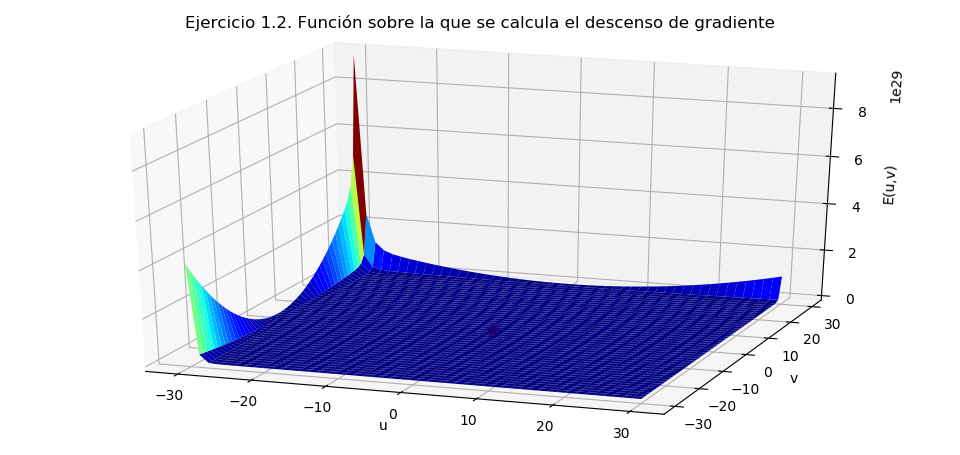
\includegraphics[scale = 0.70]{ej1-2.png}
 		 \caption{Función $E(u,v)$}
  		\label{fig:ej1-2}

\end{figure}

En esta figura vemos el punto obtenido (estrella roja cerca de las coordenadas $(0,0)$).

En principio, como veremos también en otros ejercicios, podemos creer que la tasa de aprendizaje usada $\eta = 0.1 $ es demasiado grande, pero vemos que en este caso no es así, ya que el gradiente de la función no es para nada grande en el intervalo que nos movemos (hemos comenzado en el $(1, 1)$).

\newpage

\subsection{Pruebas usando la función $F(x,y)$ dada}

De forma similar al ejercicio 1, a excepción de unos pequeños cambios, se nos pide hacer lo mismo con la siguiente función:

$$ f(x,y) = (x-2)^2 + 2(y+2)^2 + 2sin(2\pi x)sin(2 \pi y) $$

Calculando las derivadas parciales, obtenemos la función gradiente:

$$\frac{\partial  f(x,y)}{\partial x} =    2x + 4\pi cos(2\pi x)sin(2\pi y) - 4  $$

$$\frac{\partial  f(x,y)}{\partial y} =    4x + 4\pi sin(2\pi x)cos(2\pi y) + 8  $$

Quedando de la siguiente forma en Python:

\begin{lstlisting}
# Función dada en el ejercicio 1.3.
def F(x,y):
	return np.float64( (x - 2)**2 + 2 * (y + 2)**2 + 2 * np.sin(2 * np.pi * x) * np.sin(2 * np.pi * y)  ) 

#Derivada parcial de F con respecto a x
def dFx(x, y):
    return np.float64( 2*x - 4 + 4*np.pi*np.cos(2*np.pi*x)*np.sin(2*np.pi*y) )

#Derivada parcial de F con respecto a y
def dFy(x, y):
    return np.float64( 4*y + 8 + 4*np.pi*np.sin(2*np.pi*x)*np.cos(2*np.pi*y) )

#Gradiente de F
def gradF(x, y):
    return np.array([dFx(x, y), dFy(x, y)])

\end{lstlisting}

\newpage

\subsubsection{Ejecuciones con tasa de aprendizaje 0.1 y 0.01. Diferencias e importancia de la tasa de aprendizaje}


Se nos pide ejecutar el algoritmo de gradiente descendente dos veces, una con $\eta = 0.01 $ y otra con $\eta = 0.01 $, ambas con punto inicial $(1, -1)$ y con un máximo de 50 iteraciones. Como no nos especifican error, el error permitido que se le pasará a la función sera de $-\infty$ para que no lo tenga como parada, y siempre que pueda rebaje el número.

\textbf{Ejecución con $\eta = 0.01$:}

\begin{figure}[H]
  \centering
      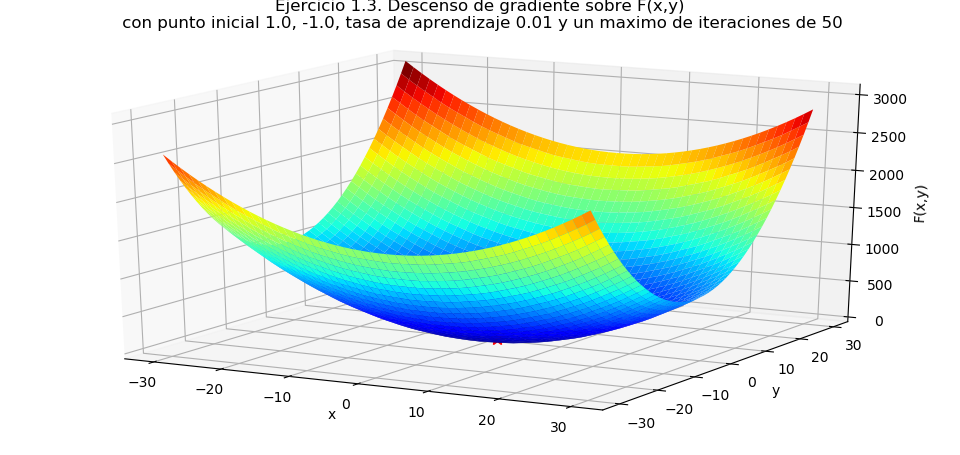
\includegraphics[scale = 0.70]{ej1-3-1-1-01.png}
 		 \caption{Función $F(x,y)$ en el punto inicial $(1,-1)$ y tasa de aprendizaje $\eta = 0.01$}
  		\label{fig:ej1-3-1-1-01}

\end{figure}

En este caso obtenemos los siguientes resultados:
\begin{lstlisting}
Valor de la función tras  49  iteraciones:  -0.3812494974381
Tasa de aprendizaje:  0.01
Error mínimo permitido:  -inf
Numero de iteraciones maximas:  50
Numero de iteraciones:  50
Coordenadas iniciales: ( 1.0 ,  -1.0 )
Coordenadas obtenidas: ( 1.269064351751895 ,  -1.2867208738332965 )
Valor de la función en dichas coordenadas -0.3812494974381
\end{lstlisting}

\newpage

Y podemos ver como avanza el valor de función con respecto a las iteraciones:

\begin{figure}[H]
  \centering
      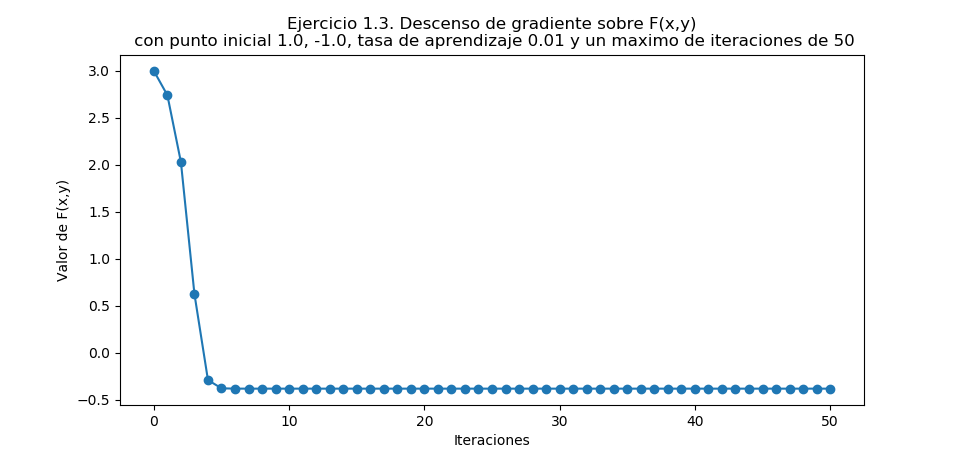
\includegraphics[scale = 0.70]{ej1-3-1-1-01-ite.png}
 		 \caption{Valor de $F(x,y)$ con tasa de aprendizaje $\eta = 0.01$, tras las distintas iteraciones}
  		\label{fig:ej1-3-1-1-01}

\end{figure}


\textbf{Ejecución con $\eta = 0.1$:}


\begin{figure}[H]
  \centering
      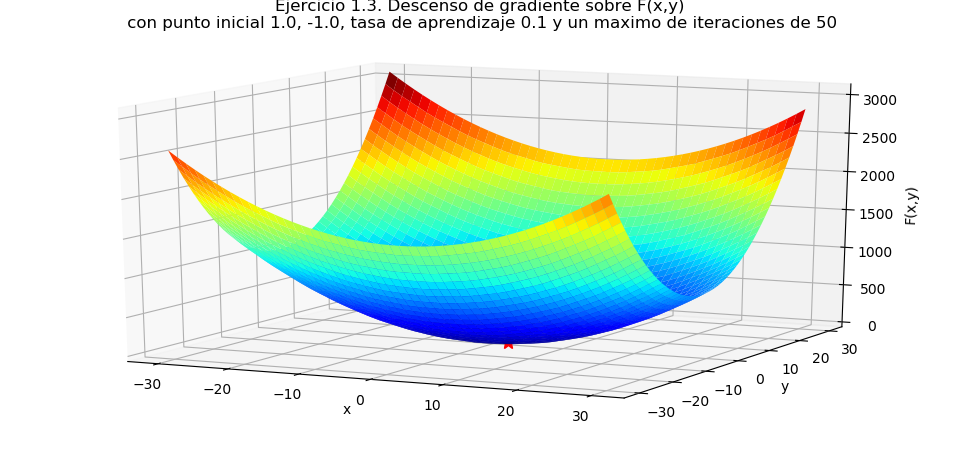
\includegraphics[scale = 0.70]{ej1-3-1-1-10.png}
 		 \caption{Función $F(x,y)$ en el punto inicial $(1,-1)$ y tasa de aprendizaje $\eta = 0.1$}
  		\label{fig:ej1-3-1-1-10}

\end{figure}

En este caso obtenemos los siguientes resultados:
\begin{lstlisting}
Tasa de aprendizaje:  0.1
Error mínimo permitido:  -inf
Numero de iteraciones maximas:  50
Numero de iteraciones:  50
Coordenadas iniciales: ( 1.0 ,  -1.0 )
Coordenadas obtenidas: ( 2.939376479816701 ,  -1.607795422435394 )
Valor de la función en dichas coordenadas 0.7241149424996057
\end{lstlisting}

Vemos como en este caso los resultados son peores, ya que obtenemos un valor mayor en las coordenadas tras 50 iteraciones. Vamos a ver como avanza el valor de la función en este caso:


\begin{figure}[H]
  \centering
      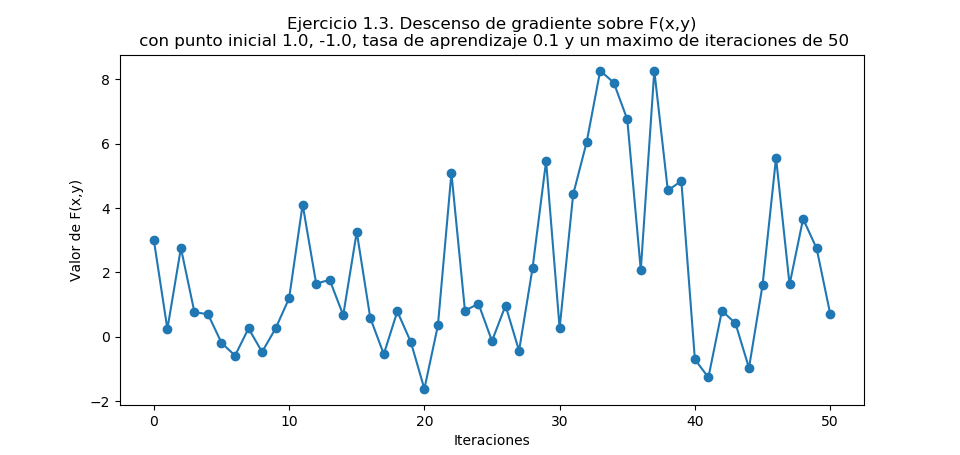
\includegraphics[scale = 0.70]{ej1-3-1-1-10-ite.png}
 		 \caption{Valor de $F(x,y)$ con tasa de aprendizaje $\eta = 0.1$, tras las distintas iteraciones}
  		\label{fig:ej1-3-1-1-10-ite}

\end{figure}


En este caso el valor de la función no se estabiliza, esto es debido a que el gradiente de la función es alto, sumado a que tenemos una mayor tasa de aprendizaje el punto se mueve demasiado dejando atrás el mínimo que antes encontraba con $\eta = 0.01$ y moviendose por toda la función. Como detalle añadir que vemos en algunas iteraciones, como la iteración número 20, que llegamos a obtener valores menores al mínimo obtenido con $\eta = 0.01$, lo que nos podría dar una pista de que el mínimo antes encontrado es un mínimo local de la función.

Esto último lo podemos ver mejor en la siguiente gráfica, en la que pintamos a la vez los valores obtenidos con ambas tasas:

\begin{figure}[H]
  \centering
      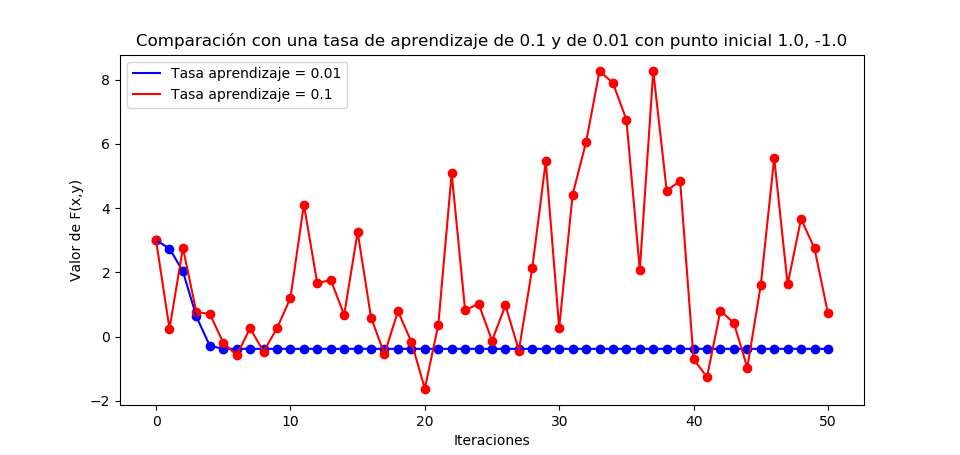
\includegraphics[scale = 0.70]{ej1-3-1-1-ite.png}
 		 \caption{Valor de $F(x,y)$ con ambas tasas de aprendizaje, tras las distintas iteraciones}
  		\label{fig:ej1-3-1-1-ite}

\end{figure}


Tras este experimento vemos la importancia de la tasa de aprendizaje, ya que escogerla mal supone que el algoritmo no funcione, y simplemente se dedique a explorar el espacio de búsqueda, en lugar de explotar la zona en la que está.

\subsubsection{Pruebas con distintos puntos de inicio}

Para este apartado se nos pide probar con distintos puntos de inicio:

\begin{itemize}
	\item $(2.1, -2.1)$
	\item $(3, -3)$
	\item $(1.5, 1.5)$
	\item $(1, -1)$
\end{itemize}

Por no alargar en vano la extensión de esta documentación, solo pondré las imágenes comparando las ejecuciones probando las tasas de aprendizaje $\eta = 0.01$ y $\eta = 0.1$.

\newpage

\textbf{Punto $(2.1, -2.1)$:}

\begin{figure}[H]
  \centering
      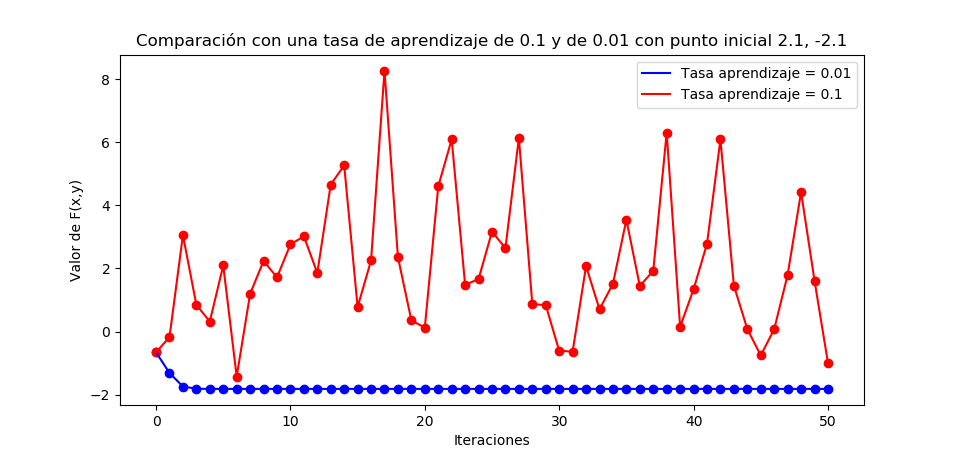
\includegraphics[scale = 0.70]{ej1-3-21-21.png}
 		 \caption{Valor de $F(x,y)$ con ambas tasas de aprendizaje, tras las distintas iteraciones}
  		\label{fig:ej1-3-21-21}

\end{figure}


\textbf{Punto $(3, -3)$:}

\begin{figure}[H]
  \centering
      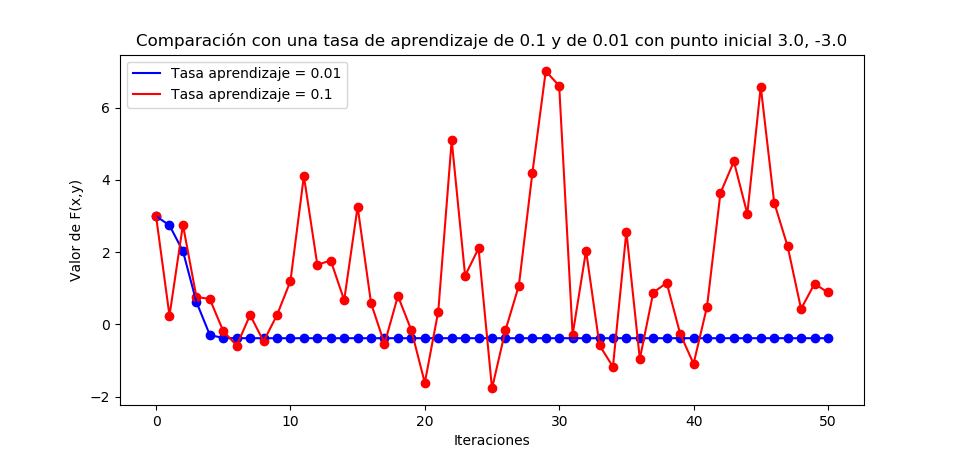
\includegraphics[scale = 0.70]{ej1-3-3-3.png}
 		 \caption{Valor de $F(x,y)$ con ambas tasas de aprendizaje, tras las distintas iteraciones}
  		\label{fig:ej1-3-3-3}

\end{figure}

\newpage

\textbf{Punto $(1.5, -1.5)$:}

\begin{figure}[H]
  \centering
      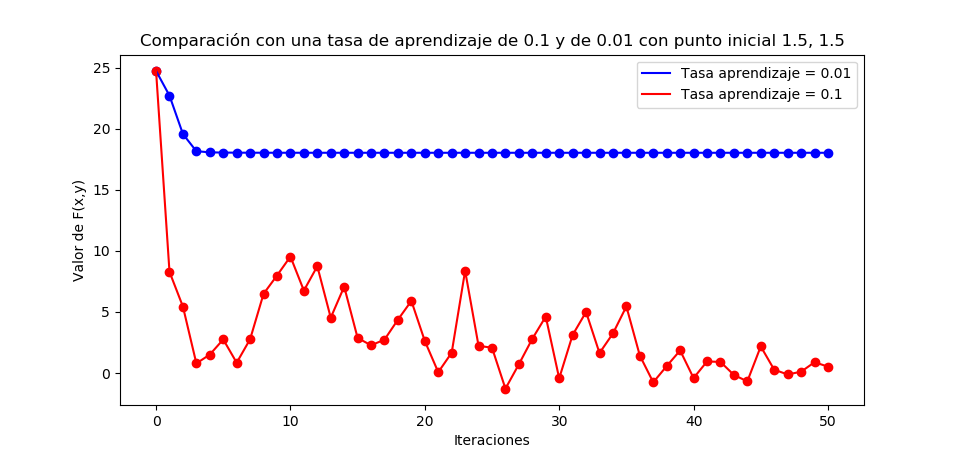
\includegraphics[scale = 0.70]{ej1-3-15-15.png}
 		 \caption{Valor de $F(x,y)$ con ambas tasas de aprendizaje, tras las distintas iteraciones}
  		\label{fig:ej1-3-15-15}

\end{figure}

En este caso me gustaría comentar el comportamiento peculiar que tiene en este caso el algoritmo con $\eta = 0.1$. Vemos como mejora mientras que $\eta = 0.01$ se queda estancado en un valor de 15. Esto se debe a que seguramente, el avance de la tasa tan pequeño le cause que encuentre un punto en el que el gradiente vale 0, y se estanque en ese punto.

\textbf{Punto $(1, -1)$:}

\begin{figure}[H]
  \centering
      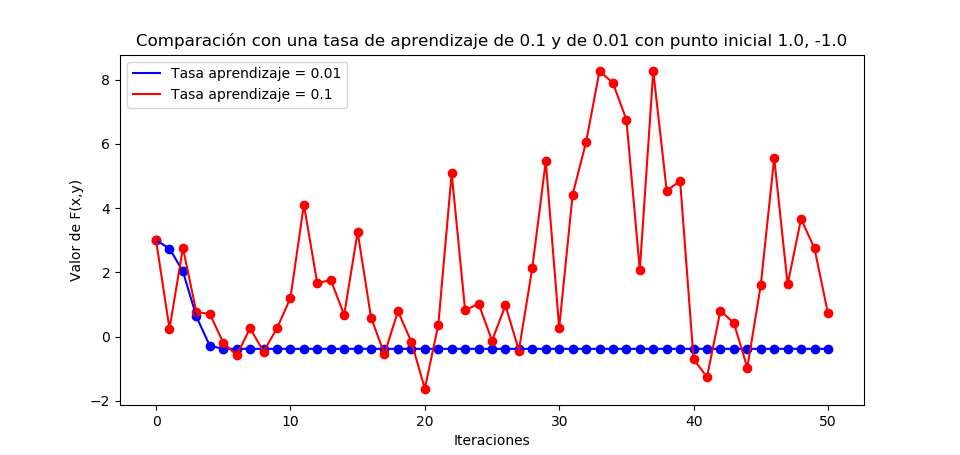
\includegraphics[scale = 0.70]{ej1-3-1-1-ite.png}
 		 \caption{Valor de $F(x,y)$ con ambas tasas de aprendizaje, tras las distintas iteraciones}
  		\label{fig:ej1-3-1-1-ite2}

\end{figure}


Vemos como en todos los casos, con $\eta = 0.1$ no se estabiliza, por lo que desechare los resultados con esta tasa de aprendizaje.

Con respecto a la tasa $\eta = 0.01$, finalmente he escogido realizar solo 50 iteraciones ya que vemos que con todos se estanca en el mismo valor con 50 iteraciones. En realidad vemos como todas se estancan con menos de 10 iteraciones, así que podríamos escoger ese límite, sin embargo como esto no afectará y ya tengo los resultados para 50 iteraciones, lo mantendré así.

\begin{table}[H]
\small
\begin{adjustwidth}{-1cm}{-1cm}%
\begin{tabular}{|c|c|c|c|c|}
\hline
\multicolumn{5}{|c|}{\textbf{Valores obtenidos con el gradiente descendente en distintos puntos}}                                                                                                                                                                                                                                                                                                                                                           \\ \hline
                                                                                          & (2.1, -2.1)                                                                            & (3, -3)                                                                                 & (1.5, -1.5)                                                                           & (1, -1)                                                                              \\ \hline
\textbf{\begin{tabular}[c]{@{}c@{}}Valor\\  mínimo\end{tabular}}                          & -1.8200785415471563                                                                    & -0.38124949743809955                                                                    & 18.042078009957635                                                                    & -0.3812494974381                                                                     \\ \hline
\textbf{\begin{tabular}[c]{@{}c@{}}Coordenadas\\ donde \\ es obtenido\end{tabular}} & \begin{tabular}[c]{@{}c@{}}( 2.2438049693647883 ,\\  -2.237925821486178 )\end{tabular} & \begin{tabular}[c]{@{}c@{}}( 2.7309356482481055 ,\\  -2.7132791261667037 )\end{tabular} & \begin{tabular}[c]{@{}c@{}}( 1.7779244744891156 ,\\  1.032056872669696 )\end{tabular} & \begin{tabular}[c]{@{}c@{}}(1.269064351751895 , \\ -1.2867208738332965)\end{tabular} \\ \hline
\end{tabular}
\end{adjustwidth}

\end{table}

\subsection{Conclusión: Verdadera dificultad para encontrar un mínimo global en una función arbitraria}

Con este ejercicio podemos ver la verdadera dificultad encontrar un mínimo global, ya que influyen distintos factores, principalmente: 


\begin{itemize}
	\item Punto de inicio
	\item Tasa de aprendizaje
	\item Gradiente de la función
\end{itemize}

El punto de inicio es importante ya que de el depende el obtener un mínimo global o uno local, a excepción de que la función sea concava en cuyo caso siempre encontrará el mínimo global, además del número de iteraciones necesarias para encontrar dicho mínimo.

La tasa de aprendizaje influye ya que de ella depende en gran parte cuanto nos movemos por la función, y si esta es muy alta, en lugar de centrarnos en una zona de la función y obtener el mínimo de esa zona, es decir, explotar la zona, podemos entrar en la situación de movernos entre distintas zonas, y posiblemente no llegar al mínimo de ninguna de estas, es decir, explorar la función.

El gradiente de la función está altamente ligado a la tasa de aprendizaje, ya que si el gradiente es muy pequeño, el tener una tasa de aprendizaje alta no afectará tanto, mientras que si es grande, el escoger una mala tasa de aprendizaje hará que se acentúen los problemas antes comentados de escogerla.

Obviamente estos factores están altamente ligados a la función a minimizar, luego depende de cada función el como escogerlos.









\section{Ejercicio sobre regresión lineal}

En el primer apartado de este ejercicio se nos dan dos conjuntos de datos (train y test) sobre características de números. Nosotros usaremos la simetría y el valor medio del nivel de gris sobre los números 1 y 5, para intentar obtener un modelo de regresión lineal a partir de train que sea capaz de clasificar el conjunto test. Para conseguir esto usaremos el método del gradiente descendente estocástico y el método de la pseudoinversa.


En todo el ejercicio intentaremos minimizar la misma función de error, que usaremos la función de mínimos cuadrados, implementada tal como se nos enseño en teoría:

$$ E (w) = \frac{1}{N}\sum_{n = 1}^{N} (w^Tx_n-y_n)^2$$ 

Implementada en Python:


\begin{lstlisting}
# Funcion para calcular el error
def Err(x,y,w):
	## Función dada en las diapositivas:
	#
	# E_in(w) = 1/N * SUM(w^T * x_n - y_n)^2
	#
	# basicamente, hacemos w * x - y al cuadrado, y le hacemos la media

	# https://docs.scipy.org/doc/numpy/reference/generated/numpy.square.html
	err = np.square(x.dot(w) - y.reshape(-1,1))

	# https://docs.scipy.org/doc/numpy/reference/generated/numpy.mean.html
	err.mean()

	return err

\end{lstlisting}

\newpage

También necesitaremos su derivada parcial, para obtener el gradiente:

$$\frac{\partial E(w)}{\partial w_j} = \frac{2}{N}\sum_{n=1}^{N} x_{nj}(h(x_n) - y_n) $$

Y su implementación en Python:

\begin{lstlisting}
def dErr(x, y, w):
	# la parte interna sigue igual
	derivada = x.dot(w) - y.reshape(-1,1)

	# el cuadrado pasa a ser un *2, y restamos una al exponente
	derivada = 2 * np.mean(x * derivada, axis=0)

	derivada = derivada.reshape(-1, 1)

	return derivada
	
\end{lstlisting}


\newpage


\subsection{Implementación y valoración del Gradiente Descendente Estocástico y el método de la Pseudoinversa}

\subsubsection{Gradiente descendente estocástico}

La filosofía del gradiente descendente estocástico es la misma que la del gradiente descendente, con la diferencia de que en este caso solo evaluaremos algunos puntos de forma aleatoria, haciendo el cálculo mucho más rápido, logrando una mayor variabilidad, además de que esto nos da evidencias empíricas de obtener un buen mínimo local en funciones no convexas\cite{teoria}.

Normalmente el tamaño de la muestra aleatoria que evaluaremos está entre 32 y 128 elementos. En la plantilla dada es usado un tamaño de 64, así que usaremos ese tamaño.

Dicho esto, el algoritmo quedará de la siguiente forma:

\begin{lstlisting}
def sgd(x, y, tasa_aprendizaje, tam_batch, maxIteraciones = 1000):
    #
	# diapositiva 17, jussto antes del metodo de newton

	# el tamaño de w será dependiendo del numero de elementos de x
	w = np.zeros((x.shape[1], 1), np.float64)

	iterations = 0

	while iterations < maxIteraciones:

		iterations = iterations + 1

		# https://docs.scipy.org/doc/numpy-1.15.0/reference/generated/numpy.random.choice.html
		# sacamos tantos indices aleatorios como tam_batch (tamaño del minibatch) queramos
		# lo sacamos a partir de la forma de x, es decir, x tendrá N filas y 1 columna
		# pues escogemos de entre las N filas tam_batch
		indices_minibatch = np.random.choice(x.shape[0], tam_batch, replace=False)

		# aplicamos la funcion dada en la diapositiva 17 del tema 1
		w = w - tasa_aprendizaje * dErr(x[indices_minibatch], y[indices_minibatch], w)

	return w, iterations
	
\end{lstlisting}


\subsubsection{Pseudoinversa}

El algoritmo de la pseudoinversa se basa en que si nosotros tenemos unos datos de entrada X y unos datos de salida Y, asociados a X, debe existir una función que aplicada a X, transforme X a Y\cite{teoria}. Nuestro objetivo será encontrar esa función de la siguiente forma, suponiendo que $w$ es la función a encontrar:

$$ wX = y $$

Entonces:

$$ w = X'y $$

Siendo $X'$ la pseudoinversa, que, como hemos visto en teoría, se calcula de la siguiente forma:

$$ X' = (X^TX)^{-1}X^T $$

Luego nuestra implementación en Python será la siguiente:

\begin{lstlisting}
# Pseudoinversa
def pseudoinverse(matriz_x, vector_y):
    #
	# https://docs.scipy.org/doc/numpy/reference/generated/numpy.transpose.html
	x_traspuesta = matriz_x.transpose()

	# cambiamos de forma Y, no sabemos cuantas filas tendrá, pero tendrá una única columna
	y_traspuesto = vector_y.reshape(-1, 1)

	# multiplicamos x por su traspuesta https://docs.scipy.org/doc/numpy/reference/generated/numpy.dot.html
	x_pseudoinversa = x_traspuesta.dot(matriz_x)

	# calculamos la inversa: https://docs.scipy.org/doc/numpy/reference/generated/numpy.linalg.inv.html
	x_pseudoinversa = np.linalg.inv(x_pseudoinversa)

	x_pseudoinversa = x_pseudoinversa.dot(x_traspuesta)

	# finalmente calculamos w con la inversa e y
	w = x_pseudoinversa.dot(y_traspuesto)

	return w
\end{lstlisting}


Aplicando ambos métodos a los conjuntos dados obtenemos:

\newpage

\textbf{Gradiente descendente estocástico:}

Como hemos visto en el ejercicio 1, la tasa de aprendizaje es muy importante a la hora de como funciona el algoritmo, de ahí que haya preferido usar $\eta = 0.01$ y darle un mayor número de iteraciones antes que escoger mal la tasa de aprendizaje. El número de iteraciones lo he escogido realizando varias ejecuciones y comprobando el punto en el que se estanca, obteniendo unas dos mil iteraciones.

Resultados:

\begin{lstlisting}
Bondad media del resultado para grad. descendente estocastico con tasa de aprendizaje 0.01, tamaño de batch de 64 y 2000 iteraciones:

Ein:  0.0816152375022607
Eout:  0.1336601662370546
\end{lstlisting}


\begin{figure}[H]
  \centering
      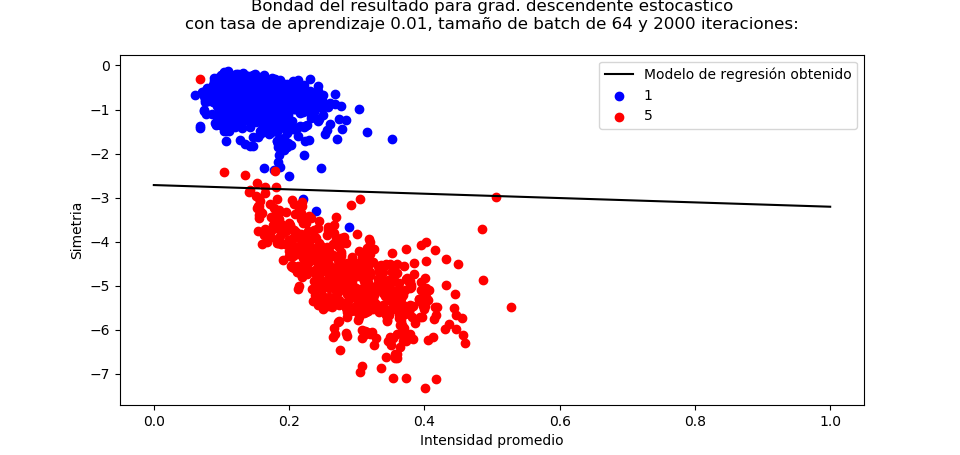
\includegraphics[scale = 0.70]{ej2-1-sgd.png}
 		 \caption{Solución con grad. descendente estocástico}
  		\label{fig:ej2-1-sgd}

\end{figure}

\begin{figure}[H]
  \centering
      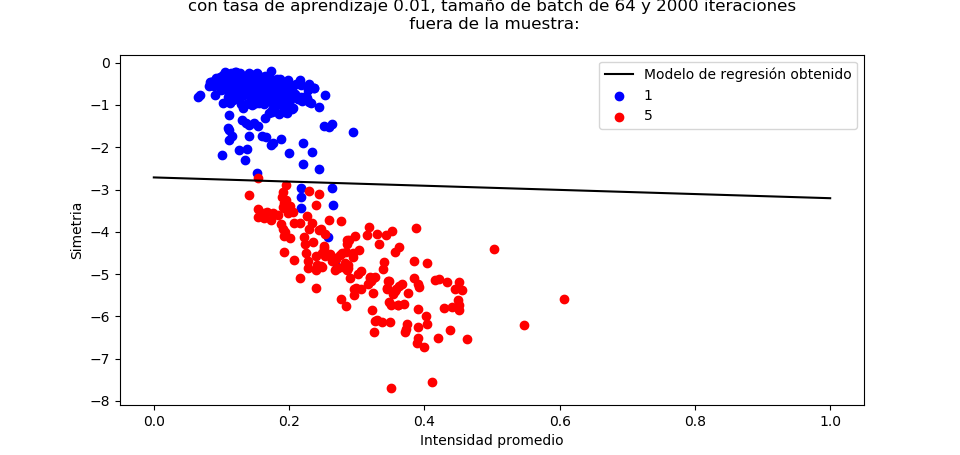
\includegraphics[scale = 0.70]{ej2-1-sgd-out.png}
 		 \caption{Probando el ajuste fuera de la muestra}
  		\label{fig:ej2-1-sgd}

\end{figure}


Vemos como $E_{in}$ y $E_{out}$ son bastante parecidos, y se ajusta bastante bien tanto dentro como fuera de la muestra, por lo que podemos considerar este como un buen método.


\vspace{2cm}

\textbf{Pseudoinversa:}

En este caso simplemente ejecutamos el algoritmo, obteniendo lo siguiente:



\begin{lstlisting}
Bondad media del resultado para pseudoinversa:

Ein:  0.07918658628900395
Eout:  0.1309538372005258
\end{lstlisting}


\begin{figure}[H]
  \centering
      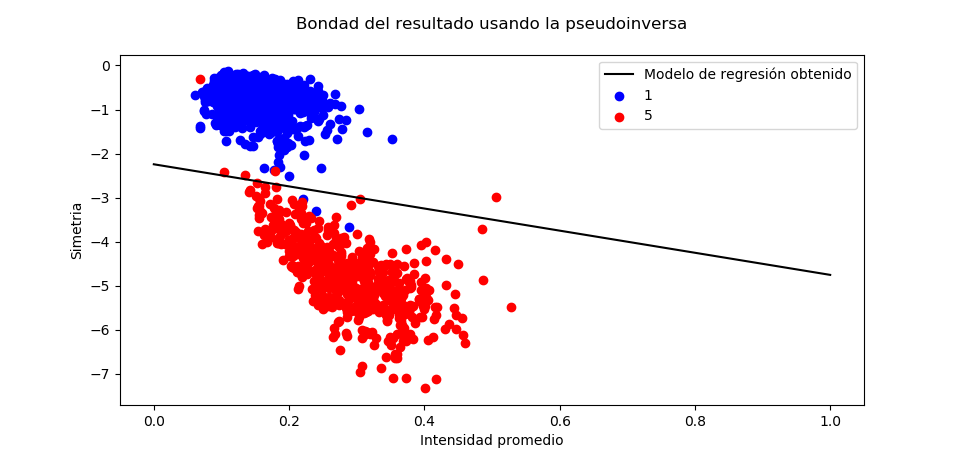
\includegraphics[scale = 0.70]{ej2-1-pseudo.png}
 		 \caption{Solución usando la pseudoinversa.}
  		\label{fig:ej2-1-pseudo}

\end{figure}

\begin{figure}[H]
  \centering
      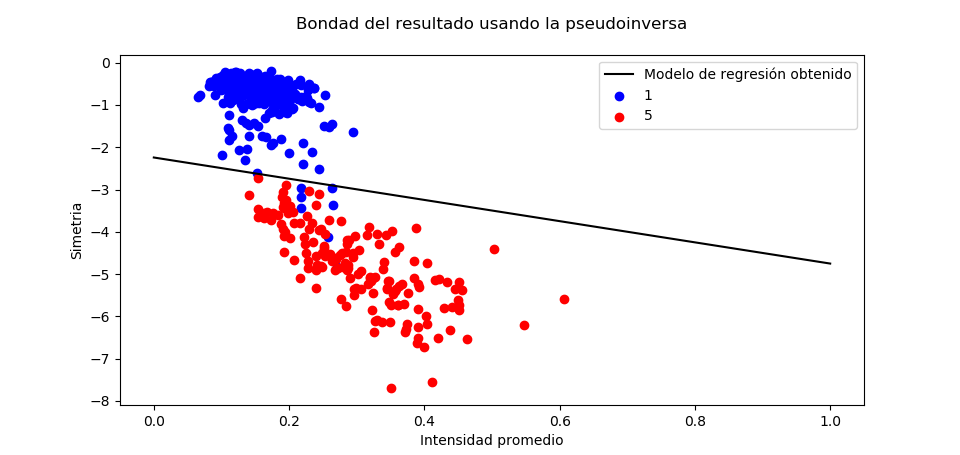
\includegraphics[scale = 0.70]{ej2-1-pseudo-out.png}
 		 \caption{Probando el ajuste fuera de la muestra}
  		\label{fig:ej2-1-pseudo-out}

\end{figure}

De nuevo vemos como este ajuste se comporta bastante bien, mejor incluso que el gradiente descendente estocastico dentro de la muestra, manteniendo el error fuera de la muestra.

\subsection{Experimento usando puntos uniformemente muestreados}

Para este ejercicio generaremos una serie de puntos uniformemente muestreados en el espacio $X = [-1, 1] x [-1, 1]$, aplicaremos a dichos puntos una función $f$ dada y tras aplicar dicha función insertaremos ruido sobre el conjunto de datos. Con este conjunto de datos intentaremos obtener modelos de regresión lineal y estimar su error usando gradiente descendente estocástico.


\textbf{Aviso:} Puede que el conjunto de datos varíe entre una captura y otra 

\begin{figure}[H]
  \centering
      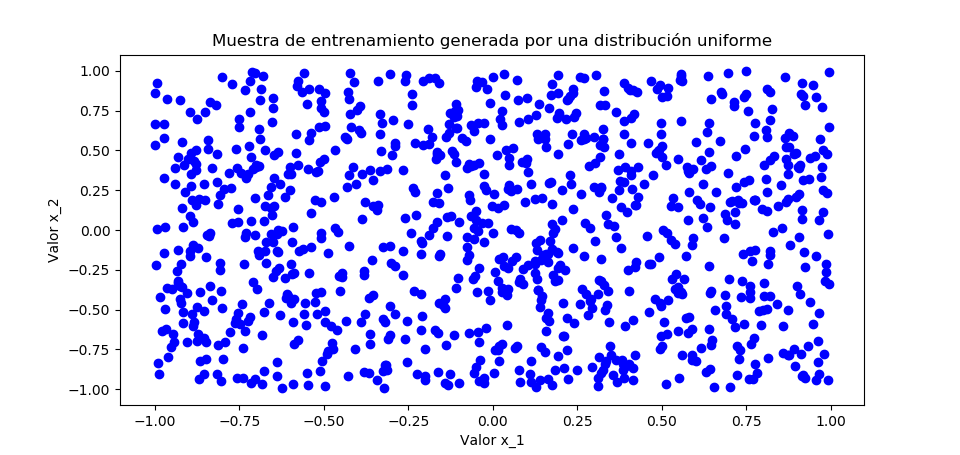
\includegraphics[scale = 0.70]{entrenamiento.png}
 		 \caption{Muestra de entrenamiento}
  		\label{fig:ej2-2-m}

\end{figure}


La función $f$ es la siguiente:

$$ f(x_1,x_2) = sign((x_1 - 0.2)^2 + x_2^2 - 0.6)  $$


\begin{figure}[H]
  \centering
      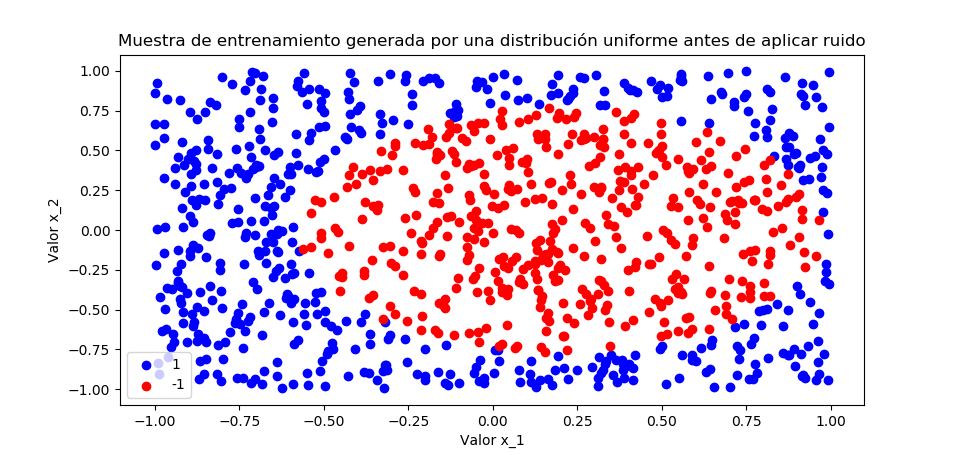
\includegraphics[scale = 0.70]{muestra-f.png}
 		 \caption{Muestra de entrenamiento tras aplicar $f$}
  		\label{fig:ej2-2-m-f}

\end{figure}

Por último, para aplicar ruido, usaremos la siguiente función que he desarrollado:

\begin{lstlisting}
# funcion para aplicar el ruido
# Parametro 1: array de etiquetas donde aplicar el ruido: suponemos que son 1/-1
# parametro 2: porcentaje de etiquetas al que aplicar el ruido
def ruido(etiquetas, porcentaje):

	n_etiquetas = etiquetas.copy()

	num_etiquetas = len(n_etiquetas)

	num_a_aplicar = num_etiquetas * porcentaje
	num_a_aplicar = int(round(num_a_aplicar))

	indices = np.random.choice(range(num_etiquetas), num_a_aplicar, replace=False)


	for i in indices:
		n_etiquetas[i] = -n_etiquetas[i]

	return n_etiquetas
\end{lstlisting}

\newpage

Vemos como su funcionamiento es simple, recibe un array de etiquetas y un porcentaje, escoge aleatoriamente y sin repeticiones a que elementos aplicar el ruido acorde al porcentaje dado, y a dichos valores les cambia el signo de la etiqueta. Esta función supone que las posibles etiquetas son 1/-1.



\begin{figure}[H]
  \centering
      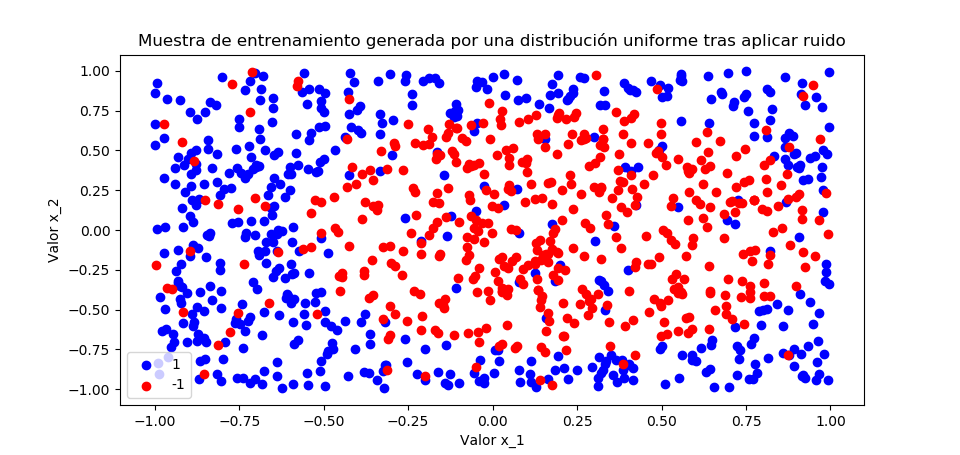
\includegraphics[scale = 0.70]{muestra-f-r.png}
 		 \caption{Muestra de entrenamiento tras aplicar $f$ y el ruido}
  		\label{fig:ej2-2-m-f=r}

\end{figure}

A partir de aquí dividiré en dos el ejercicio, ya que se nos pide realizar el experimento con características lineales y no lineales:

\newpage

\subsubsection{Usando características lineales}

Para este caso usaremos las siguientes características: $(1, x_1, x_2)$ que como vemos son lineales, es decir, el ajuste de la regresión será una linea recta la cual he dibujado obteniendo dos puntos de esta, como podemos ver:


\begin{figure}[H]
  \centering
      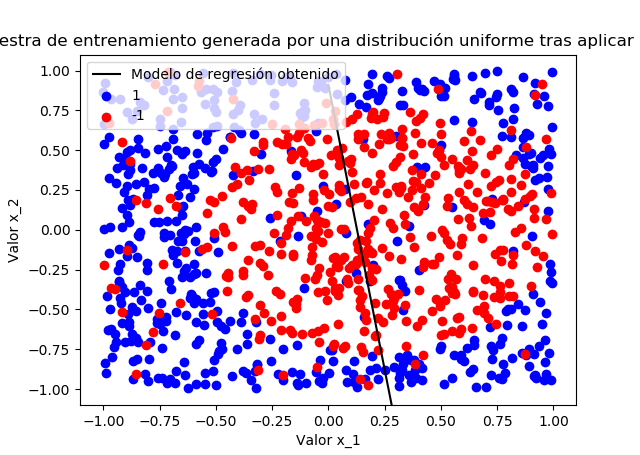
\includegraphics[scale = 0.70]{muestra-f-r-1c.png}
 		 \caption{Muestra de entrenamiento tras aplicar $f$ y el ruido mostrando el ajuste obtenido}
  		\label{fig:ej2-2-m-f-r-1c}

\end{figure}

Con este modelo obtenemos el siguiente error dentro de la muestra:

\begin{lstlisting}
Ein medio:  0.9234946965042372
\end{lstlisting}

Tras esto continuamos con el experimento, en este caso generamos 1000 muestras de entrenamiento, por cada muestra obtenemos su respectivo ajuste, y comprobamos el error fuera de la muestra con otro conjunto de test generado de la misma forma.

Para realizar estos experimentos he rebajado a 1500 el número de iteraciones para que no tarde tanto.

\newpage

\begin{lstlisting}
while total < 1000:
	if (total == 500):
		print('Llevamos la mitad, tu puedes python')
	total = total + 1
	m = simula_unif(1000, 2, 1)
	etiq = F(m[:, 0], m[:, 1])
	etiq = ruido(etiq, 0.1)
	unos = np.ones((m.shape[0], 1), dtype=np.float64)
	c = np.c_[unos, m]
	eta = 0.01
	w, iteraciones = sgd(c, etiq, eta, 64, 1500)
	Ein_ite.append(Err(c, etiq, w))

	m_out = simula_unif(1000, 2, 1)
	etiq_out = F(m_out[:, 0], m_out[:, 1])
	etiq_out = ruido(etiq_out, 0.1)
	c_out = np.c_[unos, m_out]
	Eout_ite.append(Err(c_out, etiq_out, w))
\end{lstlisting}

Finalmente, obtenemos el valor en media de los errores dentro y fuera de la muestra:

\begin{lstlisting}
Error medio dentro de la muestra:  0.9270532733520994
Error medio fuera de la muestra:  0.9328568587280501
\end{lstlisting}

\newpage

\subsubsection{Usando características no lineales}



Para este caso usaremos las siguientes características: $(1, x_1, x_2, x_1x_2, x_1^2, x_2^2)$ que como vemos son no lineales, el ajuste de la regresión no será una linea recta, será una elipse la cual he dibujado evaluando distintos puntos de la elipse haciendo uso del paquete sympy\cite{documentacion-sympy} de python:

\begin{lstlisting}
# y = w[0] + w[1]*x1 + w[2]*x2 + w[3]*x1*x2 + w[4]*x1^2 + w[5]*x2^2
# desde -1 hasta 1, el rango en el que generamos los puntos
i = -1

z = Symbol('x')

while i <= 1:
	# resolvemos la ecuacion para cada punto de i, suponiendo y = 0
	valores_funcion = solve(w[0] + w[1]*i + w[2]*z + w[3]*i*z + w[4]*i*i + w[5]*z*z, z)

	# si los valores obtenidos no son imaginarios los añadimos a los que hay que dibujar
	# (Sympy representa los imaginarios como instancia de Add)
	if not isinstance(valores_funcion[0][0], Add):
		valores_entre_cero_uno.append(i)
		valores_a_dibujar_inf.append(valores_funcion[0])
	if not isinstance(valores_funcion[1][0], Add):
		valores_a_dibujar_sup.append(valores_funcion[1])
	i = i + 1/100

\end{lstlisting}

\begin{figure}[H]
  \centering
      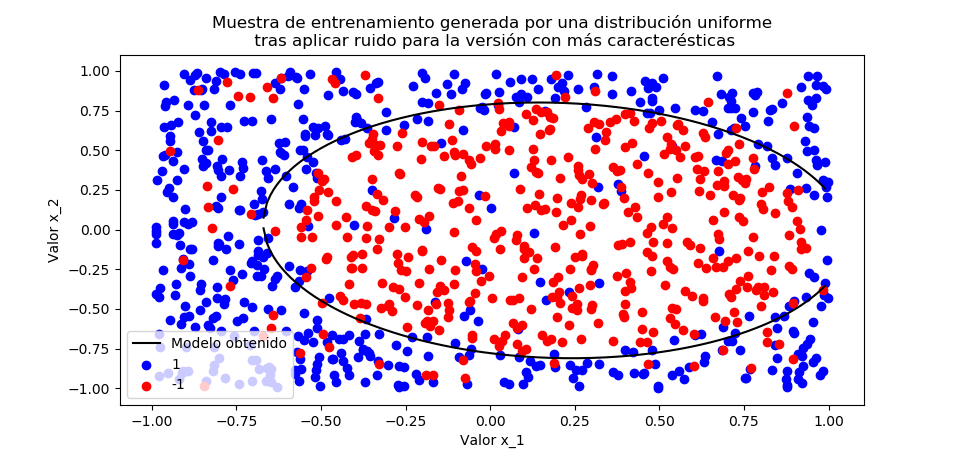
\includegraphics[scale = 0.70]{muestra-f-r-6c.png}
 		 \caption{Muestra de entrenamiento tras aplicar $f$ y el ruido mostrando el ajuste obtenido}
  		\label{fig:ej2-2-m-f-r-1c}

\end{figure}

Con este modelo obtenemos el siguiente error dentro de la muestra:

\begin{lstlisting}
Ein medio:  0.58906135748821
\end{lstlisting}

Tras esto continuamos con el experimento, en este caso generamos 1000 muestras de entrenamiento, por cada muestra obtenemos su respectivo ajuste, y comprobamos el error fuera de la muestra con otro conjunto de test generado de la misma forma.

Para realizar estos experimentos he rebajado a 1500 el número de iteraciones para que no tarde tanto.

Esto lo hacemos exactamente igual, pero con las nuevas características.

Finalmente, obtenemos el valor en media de los errores dentro y fuera de la muestra:

\begin{lstlisting}
Error medio dentro de la muestra:  0.5854493123425574
Error medio fuera de la muestra:  1.3403024104466463
\end{lstlisting}



\subsection{Diferencias entre el uso de características lineales y no lineales. Que modelo es el más adecuado}

Vemos como usando características lineales el ajuste es una recta que sitúa sobre el centro de los datos, intentando dividirla por la mitad. Esto hace que se minimice el error, sin embargo realmente no estamos consiguiendo una buena clasificación.

Haciendo uso de características no lineales vemos como el error medio dentro de la muestra es mucho menor que el error con características lineales, sin embargo fuera de la muestra se comporta bastante peor, seguramente por el ruido.

Con respecto a cual es el modelo más adecuado, de nuevo, depende de la función a ajustar, si como en este caso, la función separa el conjunto en un subconjunto, rodeado de otros valores, las características no lineales serán mejor opción, si vemos que claramente existe una división entre los valores, como en el caso del primer apartado, el uso de características lineales se ajustará mejor.

\newpage

\section{Ejercicio bonus: Método de Newton}

El método de Newton toma la misma idea que el gradiente descendente, pero con el objetivo de intentar encontrar el mínimo cuando está cerca de el, es decir, con el gradiente descendente conseguimos ir desde una zona con un valor bastante malo a una zona de un mínimo (ya sea global o local, como hemos comentado), mientras que con el método de Newton intentamos encontrar el mínimo cuando estamos ya en esa zona\cite{teoria}.

Es decir, el método de Newton solo nos funcionará para zonas cercanas al mínimo. Esto lo conseguirá haciendo uso de las derivadas parciales de segundo orden de la función a minimizar, en concreto con la matriz hessiana\cite{m-hessiana}, formada por dichas derivadas parciales de segundo orden.

También tenemos que tener en cuenta que la matriz hessiana puede ser de dos tipos:

\begin{itemize}
	\item Positiva-definida: Los menores principales de la matriz son positivos, $f$ es estrictamente convexa y alcanzaremos un mínimo local.
	\item Negativa-definida: Los menores principales de la matriz son negativos, $f$ es estrictamente cóncava y alcanzaremos un máximo local.
\end{itemize}

Ya que nosotros intentamos minimizar la función, el supondremos ambos casos, si es positiva-definida, seguiremos la matriz hessiana y nos acercaremos a un mínimo, mientras que si es negativa-definida invertiremos la suma del gradiente, alejándonos del máximo.

Es decir, nosotros intentaremos obtener el incremento de $w$:

$$ \Delta w = -H^{-1} \nabla E_{in}(w_0) $$

Donde $H$ es la siguiente matriz:


\[ H =  \left( \begin{array}{cc}
\frac{\partial^{2} f(x_1, x_2)}{\partial x_1^2} 					& \frac{\partial^{2} f(x_1, x_2)}{\partial x_1 \partial x_2} \\
\frac{\partial^{2} f(x_1, x_2)}{\partial x_1 \partial x_2} & \frac{\partial^{2} f(x_1, x_2)}{\partial x_2^2}
\end{array} \right ) \] 


Si la matriz es positiva-definida, $\Delta w$ nos acercará a un mínimo, luego $w_j$ será:

$$ w_j = w_j + \eta * \Delta w$$

Mientras que si la matriz es negativa-definida, $\Delta w$ nos acercará a un máximo, luego iremos en la dirección contraria:

$$ w_j = w_j - \eta * \Delta w$$


\subsection{Implementación del método de Newton}

Una vez vista la base teórica, para la implementación necesitaremos las segundas derivadas de $f(x_1, x_2)$. Del mismo modo que obtenía las derivadas parciales, obtengo las segundas derivadas, por no alargar más el documento no haré su desarrollo:

$$\frac{\partial^{2} f(x_1, x_2)}{\partial x_1^2} =  - 8 \pi^2 sin(2 \pi x) sin(2 \pi y) + 2$$

$$\frac{\partial^{2} f(x_1, x_2)}{\partial x_2^2} =  - 8 \pi^2 sin(2 \pi x) sin(2 \pi y) + 4$$

$$ \frac{\partial^{2} f(x_1, x_2)}{\partial x_1 \partial x_2} = 8\pi cos(2\pi x) cos(2 \pi y) $$

Con esto, definimos estas operaciones en Python de la siguiente forma:

\begin{lstlisting}
# segunda derivada parcial con respecto a x
def ddFx(x, y):
	return np.float64(-8*np.square(np.pi) * np.sin(2*np.pi*x) * np.sin(2*np.pi*y) + 2 )

# segunda derivada parcial con respecto a y
def ddFy(x, y):
	return np.float64(-8*np.square(np.pi) * np.sin(2*np.pi*x) * np.sin(2*np.pi*y) + 4 )

# segunda derivada respecto a x e y (son equivalentes a la de Y y x)
def ddF(x, y):
	return np.float64(8*np.square(np.pi) * np.cos(2*x*np.pi)*np.cos(2*y*np.pi))

# matriz hessiana
def matriz_hessiana(x, y):
	#https://en.wikipedia.org/wiki/Hessian_matrix
	return np.array([[ddFx(x,y), ddF(x,y)],[ddF(x,y), ddFy(x,y)]])
\end{lstlisting}

\newpage

Y siguiendo la explicación teórica del método de Newton, usando el añadido para intentar buscar el mínimo de la función, la implementación en Python quedaría de la siguiente forma:
\begin{lstlisting}
def metodo_newton(funcion, gradFuncion, matriz_hessiana, w_0, eta = 1, maxIter = 50):
    #metodo de newton -> diapositiva 18 de teoria
    # 
	iterations = 0
	error = funcion(w_0[0], w_0[1])
	w_j = w_0
	valores = np.array(funcion(w_j[0], w_j[1]))

	# Condición de parada, llegamos al límite de iteraciones
	while iterations < maxIter:
		# seguimos la formula dada en teoria
		hessiana_invertida = -np.linalg.inv(matriz_hessiana(w_j[0], w_j[1]))

		# si la hessiana es positiva_definida, apunta a un minimo, por lo que nos acercamos a ese mínimo
		positiva_definida = w_j + eta * hessiana_invertida.dot(gradFuncion(w_j[0], w_j[1]).reshape(-1, 1)).reshape(-1,)
		# si es negativa_definida, apunta a un máximo, por lo que nos alejamos de el
		negativa_definida = w_j - eta * hessiana_invertida.dot(gradFuncion(w_j[0], w_j[1]).reshape(-1, 1)).reshape(-1,)

		# nos quedamos con la suposición que nos minimice
		if funcion(positiva_definida[0], positiva_definida[1]) > funcion(negativa_definida[0], negativa_definida[1]):
			w_j = negativa_definida
		else:
			w_j = positiva_definida

		error = funcion(w_j[0], w_j[1])
		valores = np.append(valores, error)
		print('Valor de la función tras ', iterations, ' iteraciones: ', error )
		iterations = iterations + 1

	w = w_j
	return w, iterations, valores
\end{lstlisting}

Debido a que existen implementaciones con tasa de aprendizaje y otras sin tasa de aprendizaje, el valor por defecto de $\eta$ es 1, para que si queremos ejecutarlo sin tasa de aprendizaje no tenga efecto.

\subsection{Comparación del valor de la función tras las distintas iteraciones}

Para hacer la comparación con distintas iteraciones he ejecutado el método de Newton tres veces:

\begin{itemize}
	\item $\eta = 0.01$
	\item $\eta = 0.1$
	\item $\eta = 1$
\end{itemize}

Las dos primeras como comparación del método de Newton contra el gradiente descendente, y la última por comparar implementaciones que tiene en cuenta tasas de aprendizaje con una que no. Además, también ejecutaré el gradiente descendente con $\eta = 0.01$ para compararlo.

Para no hacer más extenso este documento pondré las gráficas comparando las 4 ejecuciones:


\begin{figure}[H]
  \centering
      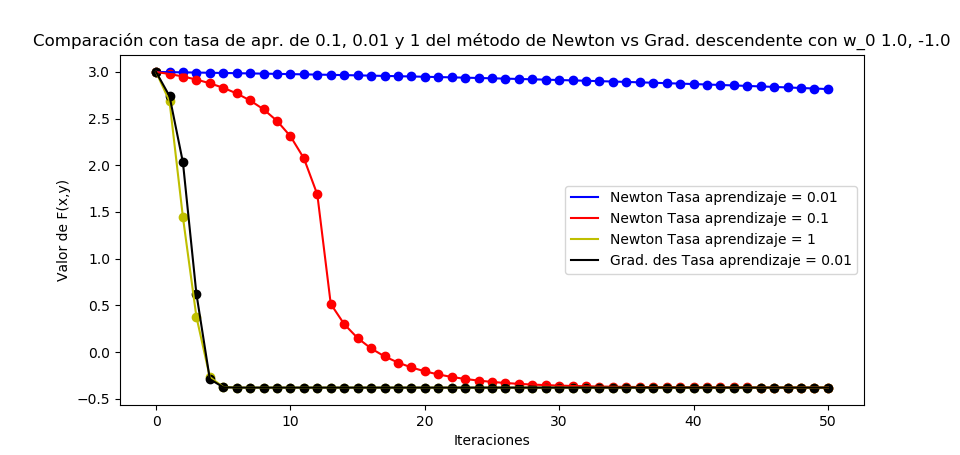
\includegraphics[scale = 0.70]{ej3-1.png}
 		 \caption{Función $F(x,y)$ en el punto inicial $(1,-1)$}
  		\label{fig:ej3-1}

\end{figure}

\begin{figure}[H]
  \centering
      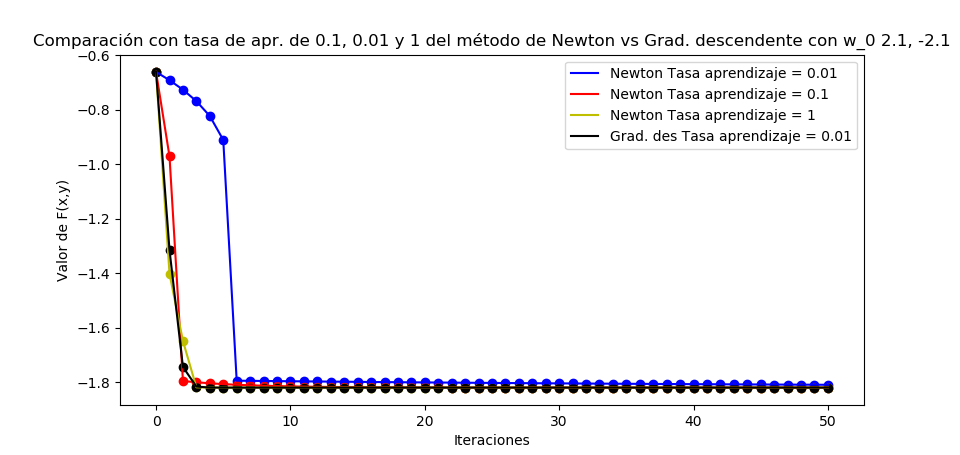
\includegraphics[scale = 0.70]{ej3-2.png}
 		 \caption{Función $F(x,y)$ en el punto inicial $(2.1,-2.1)$}
  		\label{fig:ej3-2}

\end{figure}

\begin{figure}[H]
  \centering
      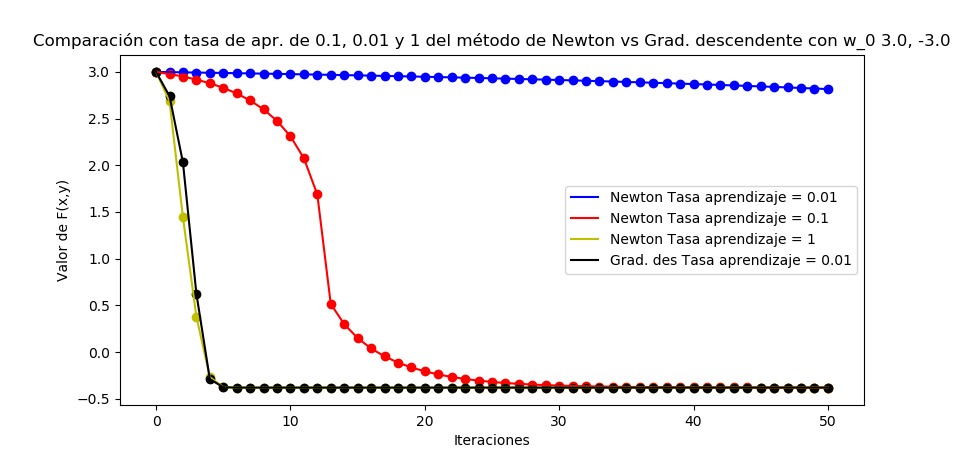
\includegraphics[scale = 0.70]{ej3-3.png}
 		 \caption{Función $F(x,y)$ en el punto inicial $(3,-3)$}
  		\label{fig:ej3-3}

\end{figure}

\begin{figure}[H]
  \centering
      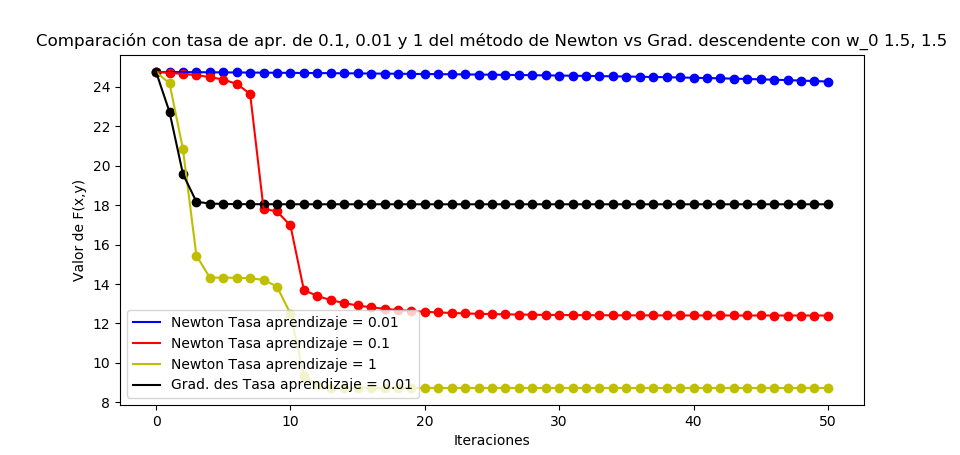
\includegraphics[scale = 0.70]{ej3-4.png}
 		 \caption{Función $F(x,y)$ en el punto inicial $(1.5,-1.5)$}
  		\label{fig:ej3-4}

\end{figure}

\subsection{Conclusiones del método de Newton y comparación con el gradiente descendente}

Como comparación podemos ver como el método de Newton es equivalente al gradiente descendente en muchos sentidos, aunque existen dos claras diferencias:

\begin{enumerate}
	\item {Tasa de aprendizaje: La tasa de aprendizaje en el método de Newton se usará para ver como de rápido avanzamos, sin embargo, no influye para obtener el mínimo como en el gradiente descendente, en el que si escogíamos mal la $\eta$ podíamos no llegar al mínimo}
	\item{Mínimo asegurado: Con el método de Newton nos aseguramos llegar al mínimo, un ejemplo es el de la última comparación, donde el gradiente descendente se estanca en el valor $f(x_1, x_2) = 18$, el método de Newton es capaz de salir de estas zonas donde se estanca la función.}
\end{enumerate}

Aunque también tiene ciertos problemas, como por ejemplo, de nuevo con la última comparación, la variación de la tasa de aprendizaje ha hecho que encuentre dos mínimos distintos.

Otra de las peculiaridades del método de Newton es que funciona especialmente bien para encontrar mínimos si están cerca, por ejemplo, en $(2.1, -2.1)$, aunque $\eta$ es muy baja, es capaz de encontrar el mínimo, cuando en otros casos necesitaríamos más iteraciones, y esto es dado al punto donde se encuentra el mínimo, que observando la tabla obtenida con el gradiente descendente, este punto está cerca del inicial.

También añadir que en nuestro caso el método de Newton se comporta bien ya que hemos tenido en cuenta que queremos minimizar, y hemos modificado el funcionamiento para que en lugar de encontrar tanto mínimos como máximos, se aleje todo lo posible de los máximos y se acerque a los mínimos.


\newpage

\section{Referencias, material y documentación usada}


\begin{thebibliography}{9}

\bibitem{teoria}
Diapositivas de teoría

\bibitem{documentacion-numpy}
Documentación de NumPy:

\url{https://docs.scipy.org/doc/numpy-1.15.0/reference/generated/numpy.random.choice.html}

\url{https://docs.scipy.org/doc/numpy/reference/generated/numpy.transpose.html}

\url{https://docs.scipy.org/doc/numpy/reference/generated/numpy.dot.html}

\url{https://docs.scipy.org/doc/numpy/reference/generated/numpy.linalg.inv.html}

\url{https://docs.scipy.org/doc/numpy/reference/generated/numpy.c_.html}

\url{https://docs.scipy.org/doc/numpy/reference/generated/numpy.square.html}

\url{https://docs.scipy.org/doc/numpy/reference/generated/numpy.mean.html}

\bibitem{documentacion-sympy}
Documentación de Sympy \url{https://docs.sympy.org/latest/modules/solvers/solvers.html}

\bibitem{m-hessiana}
Matriz Hessiana \url{https://es.wikipedia.org/wiki/Matriz_hessiana/}


\end{thebibliography}

\end{document}
